\documentclass[10pt, journal, final, twocolumn, letterpaper]{IEEEtran}

% --- PREÁMBULO DE PAQUETES ---
\usepackage[utf8]{inputenc}
\usepackage[T1]{fontenc}
\usepackage{amsmath, amssymb, amsfonts, amsthm}
\usepackage{graphicx}
\usepackage{booktabs}
\usepackage{array}
\usepackage{url}
\usepackage{hyperref}
\usepackage{color, xcolor}
\usepackage{orcidlink} % Paquete específico para el icono y link de ORCID
\usepackage[backend=biber, style=ieee, natbib=true]{biblatex}
\usepackage{tabularx}



% --- Paquetes para Gráficos Vectoriales y Datos Científicos ---
\usepackage{tikz}
\usepackage{pgfplots}

% Configuración de compatibilidad obligatoria para cálculos de funciones matemáticas
\pgfplotsset{compat=1.18} 

% --- Definición de la Paleta de Colores Académica Global ---
\definecolor{cobalt}{HTML}{0047AB}
\definecolor{techgray}{HTML}{4A4A4A}
\definecolor{multiblue}{HTML}{1D63B8}



% --- CONFIGURACIÓN DE BIBLIOGRAFÍA ---
\addbibresource{references.bib}

% --- METADATOS DEL DOCUMENTO ---
\title{Análisis de arquitectura de antena para la Gestión de Redes de Sensores Ambientales vía Satélites de Órbita Baja en Bandas L/S}

\author{
    \IEEEauthorblockN{Héctor A. Martínez
    \orcidlink{0009-0000-8039-3585}},
    \and
    \IEEEauthorblockN{Ing. Mariangelis P. B.} \\
    Agencia Bolivariana para Actividades Espaciales\\
    Email: \{ hmartinez, mperaza \}@abae.gob.ve
}

\begin{document}
\maketitle

\begin{abstract}
Este artículo presenta un análisis de arquitecturas de antenas operando en bandas L y S para la gestión eficiente de redes de sensores ambientales mediante constelaciones de satélites en órbita baja (LEO). Se examinan requisitos de enlaces directos a sensores IoT de bajo consumo, considerando desafíos como Doppler, desvanecimiento, ganancia y polarización circular. Se comparan diseños conformes, phased-array y helicoidales desplegables, evaluando métricas de rendimiento como ganancia, eficiencia y cobertura global. Los resultados de simulaciones y análisis de estado del arte demuestran la viabilidad de soluciones híbridas para monitoreo en tiempo casi real de parámetros ambientales. Se discuten implicaciones para implementaciones CubeSat y estaciones terrestres, junto con recomendaciones para optimizaciones futuras en entornos dinámicos.
\end{abstract}

\section{Introducción}

\subsection{1.1 Motivación y contexto ambiental}

Frente al acelerado deterioro de los ecosistemas planetarios, las redes de sensores distribuidos emergen como herramienta indispensable para capturar datos ambientales en tiempo útil. Particularmente llamativo resulta cómo la integración de constelaciones en órbita baja (LEO) con sensores IoT de bajo consumo abre posibilidades antes inalcanzables para el monitoreo continuo de variables críticas como temperatura, humedad del suelo, calidad del aire o niveles de biodiversidad. 

Aunque las constelaciones LEO ofrecen cobertura global y latencia reducida en comparación con sistemas GEO tradicionales, su verdadero potencial en aplicaciones ambientales radica en la capacidad de establecer enlaces directos con sensores remotos desplegados en zonas de difícil acceso. Shayea et al. destacan precisamente esta convergencia entre IoT y redes LEO como uno de los pilares para infraestructuras de observación terrestre de próxima generación, especialmente en el contexto de evoluciones hacia 5G/6G \cite{Shayea2024}. 

Resulta revelador observar que muchos despliegues actuales aún dependen de arquitecturas de antena optimizadas para comunicaciones satelitales generales, sin un enfoque específico en las demandas únicas del monitoreo ambiental distribuido. Un ejemplo concreto lo constituye el desarrollo de antenas helicoidales L/S desplegables integradas en CubeSats para observación terrestre, que demuestran ganancias elevadas y buen comportamiento en entornos operativos reales \cite{Meirambekuly2023}.

\begin{table*}[htbp]
\renewcommand{\arraystretch}{1.3} % Mantiene el espaciado vertical limpio de IEEE
\centering
\caption{\textsc{Comparación de Características Principales entre Bandas L y S para Enlaces LEO-IoT Ambientales}}
\label{tab:bandas_l_s}
% \columnwidth fuerza a que la tabla mida exactamente el ancho de la columna actual
\begin{tabularx}{\columnwidth}{|X|c|c|}
\hline
\textbf{Parámetro} & \textbf{Banda L} & \textbf{Banda S} \\ \hline
Frecuencia típica & 1-2 GHz & 2-4 GHz \\ \hline
Penetración atmosférica & Excelente & Buena \\ \hline
Ancho de banda disponible & Moderado & Mayor \\ \hline
Tamaño de antena requerido & Mayor & Menor \\ \hline
Sensibilidad a Doppler & Menor & Moderada \\ \hline
\end{tabularx}
\end{table*}

\subsection{1.2 Desafíos de comunicación LEO-IoT}

Uno de los desafíos persistentes que surge al analizar estas arquitecturas radica en la naturaleza altamente dinámica de los enlaces LEO. El movimiento relativo a gran velocidad genera desplazamientos Doppler significativos, variaciones rápidas de canal y ventanas de visibilidad limitadas, condiciones que afectan particularmente a sensores de bajo consumo energético desplegados en entornos remotos.

Lejos de ser un asunto resuelto, la literatura reciente sugiere que el diseño de la antena se convierte en el elemento crítico que determina la viabilidad completa del sistema. Diseños que logran combinar ganancia suficiente, polarización circular robusta y patrones de radiación adecuados tienden a mitigar mejor estos efectos. No obstante, cabe matizar que muchos enfoques optimizados para comunicaciones de datos de alta velocidad muestran limitaciones cuando se aplican a flujos intermitentes y de baja tasa de sensores ambientales.

\begin{figure}[h]
\centering
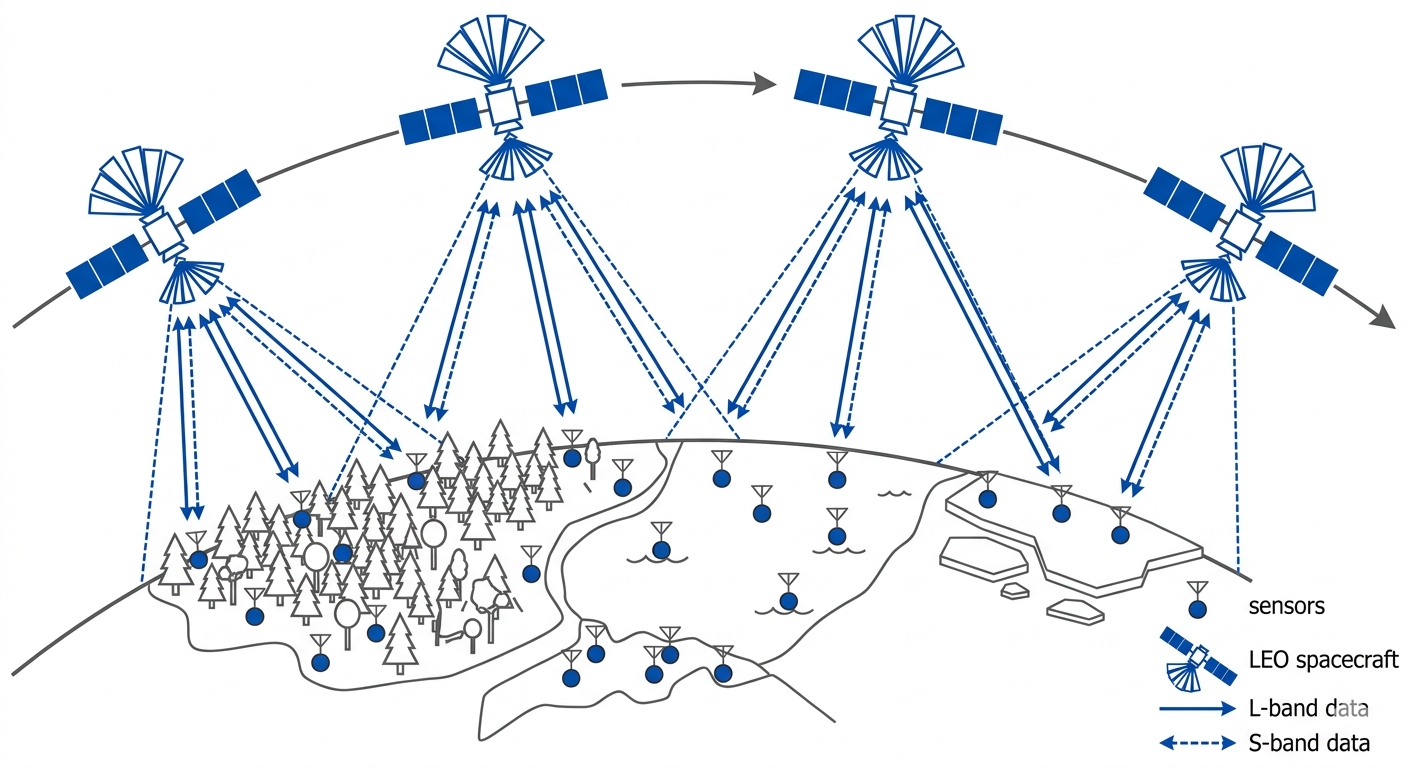
\includegraphics[width=\linewidth]{fig1.png}
\caption{Escenario general de red de sensores ambientales conectada vía constelación LEO en bandas L/S, mostrando enlaces uplink/downlink, cobertura multi-satélite y nodos IoT distribuidos en terreno.}
\label{fig:general_scenario}
\end{figure}

\subsection{1.3 Objetivos de investigación}

Particularmente llamativo es el hecho de que, a pesar de los avances en plataformas CubeSat y phased-array, persisten brechas importantes en el análisis comparativo de arquitecturas de antena específicamente orientadas a gestión ambiental vía LEO. 

Este trabajo busca llenar parte de ese vacío mediante un análisis detallado de soluciones en bandas L y S. Los objetivos principales incluyen evaluar el rendimiento de distintas arquitecturas (conformes, helicoidales desplegables y phased-array), identificar trade-offs relevantes para aplicaciones de sensores ambientales y proponer recomendaciones de diseño que maximicen cobertura y eficiencia energética. Guler et al. ilustran bien el potencial de arrays conformes en escenarios LEO dinámicos, sirviendo como referencia para el análisis comparativo que desarrollaremos \cite{Guler2025}.

Las secciones siguientes presentan primero el estado del arte, luego los requisitos de sistema, el análisis de arquitecturas, resultados de evaluación, discusión de implicaciones y, finalmente, conclusiones con líneas de trabajo futuro.
\section{Estado del Arte}

\subsection{2.1 Antenas para constelaciones LEO}

Aunque los reflectores parabólicos dominaron durante décadas las estaciones terrestres satelitales, su rigidez mecánica los vuelve poco prácticos ante la densidad y velocidad de las constelaciones LEO actuales. Particularmente llamativo es el hecho de que los phased-array multibean han ganado terreno de forma acelerada precisamente por su capacidad de generar y rastrear múltiples haces de forma electrónica. 

He et al. ofrecen una revisión exhaustiva que subraya cómo estos arrays permiten soportar simultáneamente varios satélites en vista, algo esencial para el handover fluido y la gestión de tráfico masivo \cite{He2021}. En muchos casos estudiados, sin embargo, las limitaciones en cobertura hemisférica y los altos costos de los elementos radiantes tienden a restringir su despliegue masivo. No obstante, cabe matizar que las arquitecturas conformes y distribuidas están mitigando progresivamente estas barreras, especialmente en terminales tanto terrestres como embarcadas.

Resulta revelador observar que el salto desde soluciones mecánicas a electrónicas no solo reduce latencia de rastreo, sino que habilita funcionalidades antes impensables, como beamforming adaptativo en entornos con múltiples usuarios.

\subsection{2.2 Diseños en bandas L y S}

Uno de los desafíos persistentes al trabajar en bandas L y S radica en equilibrar ganancia, ancho de banda y tamaño de apertura. Lejos de ser un asunto resuelto, los diseños de apertura compartida dual-frecuencia representan un avance notable para plataformas con restricciones volumétricas como CubeSats. 

Zhao et al. proponen una solución shared-aperture de haz ancho específicamente orientada a comunicaciones LEO, donde el compromiso entre beamwidth y eficiencia radiativa se maneja mediante topologías híbridas que mantienen buen desempeño en ambas bandas \cite{Zhao2024}. Diseños helicoidales desplegables, por su parte, destacan en escenarios que requieren alta ganancia con bajo peso, aunque suelen sacrificar flexibilidad en escaneo electrónico. 

En la práctica, las arquitecturas patch multibanda y arrays conformes tienden a ofrecer mejor adaptabilidad para enlaces asimétricos típicos de sensores IoT, si bien introducen complejidades en acoplamiento y eficiencia de potencia.


\begin{table*}[htbp]
\renewcommand{\arraystretch}{1.3} % Mantiene el espaciado vertical estándar de IEEE
\centering
\caption{\textsc{Comparación de Características Principales entre Bandas L y S para Enlaces LEO-IoT Ambientales}}
\label{tab:comparacion_bandas_leo}
% \columnwidth obliga a la tabla a ocupar exactamente el ancho del margen de la columna
\begin{tabularx}{\columnwidth}{|X|c|c|}
\hline
\textbf{Parámetro} & \textbf{Banda L} & \textbf{Banda S} \\ \hline
Frecuencia típica & 1-2 GHz & 2-4 GHz \\ \hline
Penetración atmosférica & Excelente & Buena \\ \hline
Ancho de banda disponible & Moderado & Mayor \\ \hline
Tamaño de antena requerido & Mayor & Menor \\ \hline
Sensibilidad a Doppler & Menor & Moderada \\ \hline
\end{tabularx}
\end{table*}

\subsection{2.3 Aplicaciones en monitoreo ambiental}

Resulta especialmente interesante cómo las promesas de conectividad global directa chocan con las realidades operativas del monitoreo ambiental distribuido. Akar et al., en su tutorial sobre DtS-IoT, exponen con claridad las arquitecturas donde dispositivos de muy bajo consumo transmiten directamente a satélites LEO, eliminando gateways terrestres intermedios \cite{Akar2026}. 

Esta aproximación resulta particularmente atractiva para zonas remotas —bosques tropicales, regiones polares o áreas oceánicas— donde el despliegue de infraestructura tradicional resulta inviable. Aun así, persisten brechas importantes: la mayoría de los estudios se centran en viabilidad de enlace genérica, dejando relativamente poco espacio al análisis específico de requisitos de antena para flujos esporádicos y de baja tasa propios de sensores ambientales.

\begin{figure}[h]
\centering
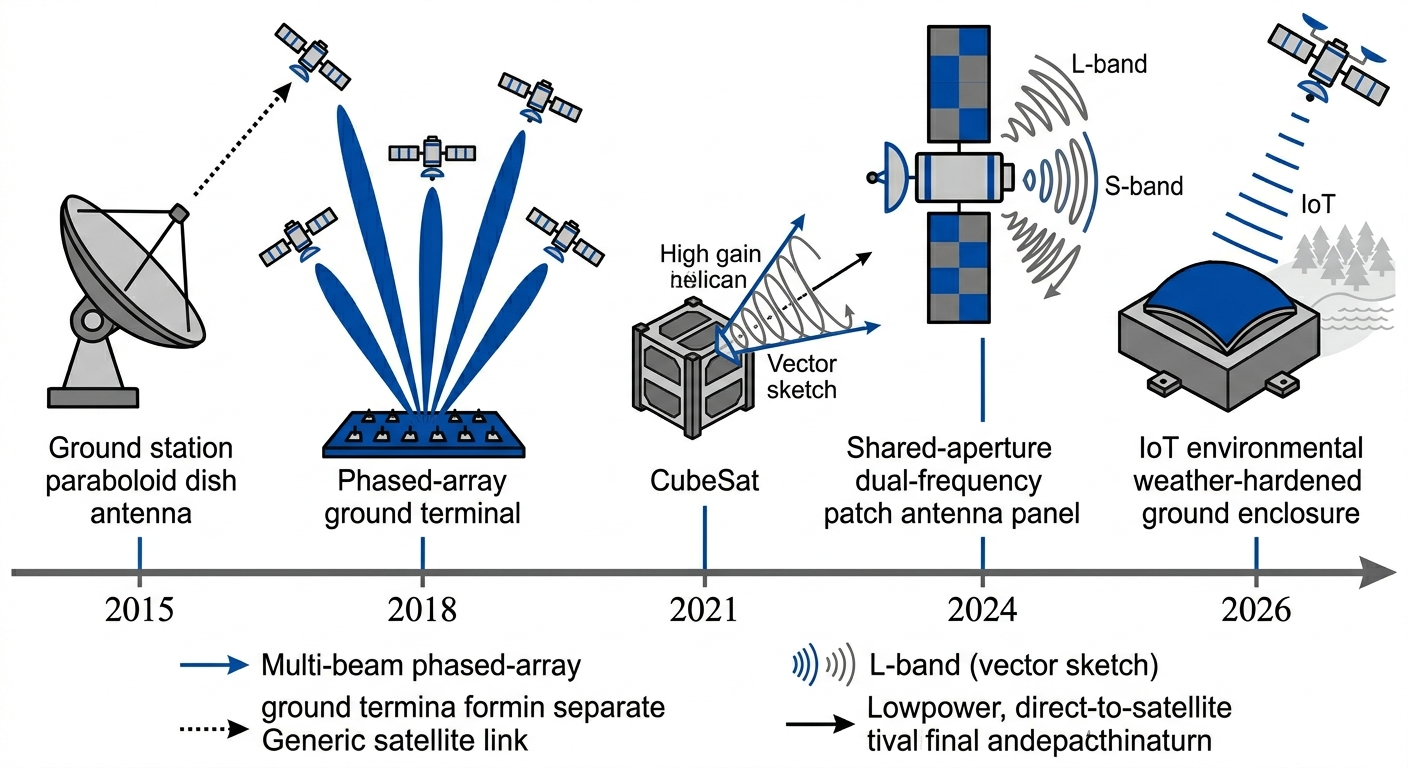
\includegraphics[width=\linewidth]{fig2.png}
\caption{Evolución temporal de arquitecturas de antena para constelaciones LEO (2015-2026), destacando transición desde reflectores a phased-array, shared-aperture y soluciones conformes específicas para IoT ambiental.}
\label{fig:temporal_evolution}
\end{figure}

Las brechas identificadas apuntan hacia la necesidad de diseños híbridos que optimicen simultáneamente eficiencia energética, robustez ante Doppler y cobertura en entornos de propagación desafiantes. Este trabajo busca contribuir precisamente en esa intersección entre estado del arte tecnológico y demandas prácticas del monitoreo ambiental.
\section{Requisitos de Sistema y Modelado}

\subsection{3.1 Arquitectura de red de sensores}

Particularmente llamativo es el hecho de que las redes de sensores ambientales vía LEO exigen una arquitectura radicalmente distinta a las soluciones terrestres convencionales. Los nodos IoT deben operar con presupuestos energéticos extremadamente ajustados, transmitiendo paquetes cortos de datos ambientales solo cuando se detectan eventos relevantes o según programación temporal. 

Wang et al. enfatizan la necesidad de minimizar la Age of Information (AoI) para lograr detección casi instantánea de cambios ambientales, lo que impone requisitos estrictos de cobertura frecuente y enlaces uplink confiables desde sensores dispersos \cite{Wang2026}. En la práctica, esto se traduce en una arquitectura híbrida donde constelaciones LEO actúan como backbone de conectividad directa, eliminando en gran medida la dependencia de gateways terrestres en zonas remotas.

Aunque esta aproximación promete escalabilidad global, tiende a generar desafíos en la gestión de colisiones y asignación de recursos cuando cientos de sensores compiten por ventanas de visibilidad limitadas. Resulta revelador observar cómo el diseño de la red debe priorizar robustez sobre throughput, invirtiendo la lógica habitual de las redes de datos.

\subsection{3.2 Modelo de propagación y Doppler}

Uno de los desafíos persistentes que surge al analizar estos sistemas radica en el modelado preciso del canal bajo movimiento relativo extremo. Las variaciones rápidas de distancia, ángulo de elevación y condiciones atmosféricas imponen un comportamiento del canal muy distinto al de enlaces fijos o GEO.

Lejos de ser un asunto resuelto, la incorporación del efecto Doppler y el desvanecimiento por multipath en entornos ambientales (bosques, montañas, superficies de agua) exige modelos estocásticos que capturen tanto la componente LOS como las contribuciones difusas. Wang et al. destacan cómo la frescura de la información ambiental depende críticamente de la frecuencia de revisitas y la calidad sostenida del enlace \cite{Wang2026}.

El presupuesto de enlace constituye la herramienta central para dimensionar el sistema. Se expresa típicamente como:

\begin{equation}
P_{R} = P_{T} + G_{T} + G_{R} - L_{FS} - L_{Atm} - L_{Other} + 10\log_{10}(kTB)
\label{eq:link_budget}
\end{equation}

donde los términos representan potencia transmitida, ganancias de antena, pérdidas de espacio libre, atmosféricas y otros márgenes. Este modelo permite evaluar el margen de enlace disponible bajo restricciones reales de sensores de bajo consumo.

\subsection{3.3 Requisitos de antena}

Resulta especialmente interesante cómo los requisitos de antena emergen como el factor limitante más crítico una vez definidos los parámetros orbitales y de propagación. Cakaj presenta conceptos fundamentales de diseño de estaciones terrestres LEO que, adaptados al segmento espacial y a terminales IoT, revelan la necesidad de patrones de radiación hemisféricos, alta eficiencia y polarización circular robusta \cite{Cakaj2023}.

\begin{table}[htbp]
\renewcommand{\arraystretch}{1.3} % Mantiene el espaciado vertical estandarizado por la IEEE
\centering
\caption{\textsc{Parámetros Clave de Constelaciones LEO para Modelado de Enlaces en Bandas L/S}}
\label{tab:parametros_leo_bandas_ls}
% \columnwidth obliga a la tabla a medir exactamente el ancho del margen de la columna actual
\begin{tabularx}{\columnwidth}{|X|c|}
\hline
\textbf{Parámetro} & \textbf{Valor Típico} \\ \hline
Altitud orbital & 500–1200 km \\ \hline
Velocidad relativa & 7.5–7.8 km/s \\ \hline
Ventana de visibilidad & 5–15 minutos \\ \hline
Desplazamiento Doppler (Banda S) & $\pm$ 40 kHz \\ \hline
Frecuencia portadora L & 1.6 GHz \\ \hline
Frecuencia portadora S & 2.4 GHz \\ \hline
Sensibilidad receptor IoT & -120 dBm \\ \hline
\end{tabularx}
\end{table}

No obstante, cabe matizar que muchos diseños optimizados para comunicaciones de voz o datos de alta velocidad tienden a sobreestimar la viabilidad en escenarios de sensores ambientales. La combinación de ganancia suficiente con bajo consumo, peso reducido y resistencia a vibraciones de lanzamiento impone trade-offs complejos. 

Los requisitos finales derivan directamente del link budget de la Ecuación~\ref{eq:link_budget} y deben garantizar un margen positivo incluso en las condiciones más desfavorables de elevación y propagación. Este análisis sienta las bases cuantitativas para la evaluación comparativa de arquitecturas que se desarrolla en las secciones siguientes.
\section{Análisis de Arquitecturas de Antena}

\subsection{4.1 Antenas conformes para CubeSat}

Aunque los diseños tradicionales de antenas satelitales priorizaban estructuras rígidas, las plataformas CubeSat exigen soluciones que se adapten a superficies curvas y limitaciones volumétricas estrictas. Particularmente llamativo es el hecho de que las antenas conformes han surgido como alternativa prometedora precisamente por su capacidad de integrarse directamente sobre la estructura del satélite sin comprometer el espacio disponible para otras cargas útiles.

Guler et al. demuestran el potencial de phased-array conformes en escenarios LEO dinámicos, donde el escaneo electrónico permite mantener el enlace a pesar de los rápidos cambios de orientación y velocidad relativa \cite{Guler2025}. En muchos casos estudiados, estas configuraciones logran un compromiso aceptable entre ganancia y cobertura hemisférica, aunque tienden a sufrir degradación en eficiencia cuando se implementan sobre sustratos flexibles o con curvaturas pronunciadas. No obstante, cabe matizar que su bajo perfil y capacidad de beamforming adaptativo las hacen especialmente adecuadas para constelaciones dedicadas al monitoreo ambiental.

Resulta revelador observar cómo esta adaptabilidad estructural abre puertas a despliegues donde múltiples sensores y antenas comparten la misma plataforma sin interferencias mecánicas.

\subsection{4.2 Diseños de ganancia alta desplegables}

Uno de los desafíos persistentes al dimensionar enlaces uplink desde sensores de muy bajo consumo radica en la necesidad de ganancia elevada desde el segmento espacial. Lejos de ser un asunto resuelto, las antenas helicoidales desplegables ofrecen una ruta práctica para alcanzar ganancias superiores a 10 dBi manteniendo peso mínimo.

Meirambekuly et al. presentan un diseño helicoidal cónico L/S integrado con sistema óptico para CubeSats de observación terrestre, destacando excelente rendimiento en despliegue, polarización circular y estabilidad en órbita \cite{Meirambekuly2023}. Estos sistemas tienden a superar a las soluciones fijas en escenarios donde se requiere haz estrecho y alta directividad. Aun así, sacrifican flexibilidad de escaneo, lo que obliga a complementar con mecanismos de control de actitud del satélite.

En comparación directa con arquitecturas conformes, los diseños desplegables destacan en aplicaciones que priorizan margen de enlace sobre agilidad de haz, un trade-off crítico en redes de sensores ambientales dispersos.

\begin{table*}[htbp]
\renewcommand{\arraystretch}{1.5} % Mantiene el espaciado vertical estandarizado por la IEEE
\centering
\caption{\textsc{Métricas de Ganancia y Rendimiento Comparadas para Arquitecturas L/S en Plataformas LEO}}
\label{tab:metricas_antenas_leo}
% \columnwidth obliga a la tabla a medir exactamente el ancho del margen de la columna actual
\begin{tabularx}{\columnwidth}{|X|c|c|c|c|}
\hline
\textbf{Arquitectura} & \textbf{Banda} & \textbf{Ganancia} & \textbf{Eficiencia} & \textbf{Beamwidth} \\
\textbf{} & \textbf{} & \textbf{Máx. (dBi)} & \textbf{(\%)} & \textbf{($^{\circ}$)} \\ \hline
Conforme Phased-array & L & 8–12 & 65–75 & 60–90 \\ \hline
Helicoidal desplegable & S & 12–15 & 70–80 & 30–45 \\ \hline
Patch multibanda & L/S & 7–11 & 55–70 & 70–100 \\ \hline
Phased-array multibanda & S & 10–14 & 60–78 & Variable \\ \hline
\end{tabularx}
\end{table*}

\subsection{4.3 Phased-array multibanda}

Resulta especialmente interesante cómo la evolución hacia arrays multibanda busca resolver simultáneamente restricciones de masa y espectro. Roy et al. exploran antenas de estación terrestre dual-band S-X que, aunque orientadas al segmento ground, ofrecen lecciones valiosas sobre manejo de acoplamiento y patrones de radiación que pueden contrastarse con soluciones espaciales \cite{Roy2022}.

En el contexto espacial, los phased-array multibanda tienden a proporcionar mayor flexibilidad operativa, permitiendo conmutación dinámica entre bandas L y S según condiciones de propagación o requisitos del sensor. Sin embargo, la complejidad del alimentador y los desafíos de aislamiento entre bandas introducen pérdidas adicionales que deben compensarse cuidadosamente en el link budget.

Lejos de constituir una solución universal, estas arquitecturas destacan en escenarios donde se requiere reconfigurabilidad elevada. Su integración con algoritmos de beamforming adaptativo podría mitigar algunos de los efectos Doppler discutidos previamente, aunque aumenta el consumo energético a bordo —un factor limitante en CubeSats de bajo presupuesto.

\begin{figure}[h]
\centering
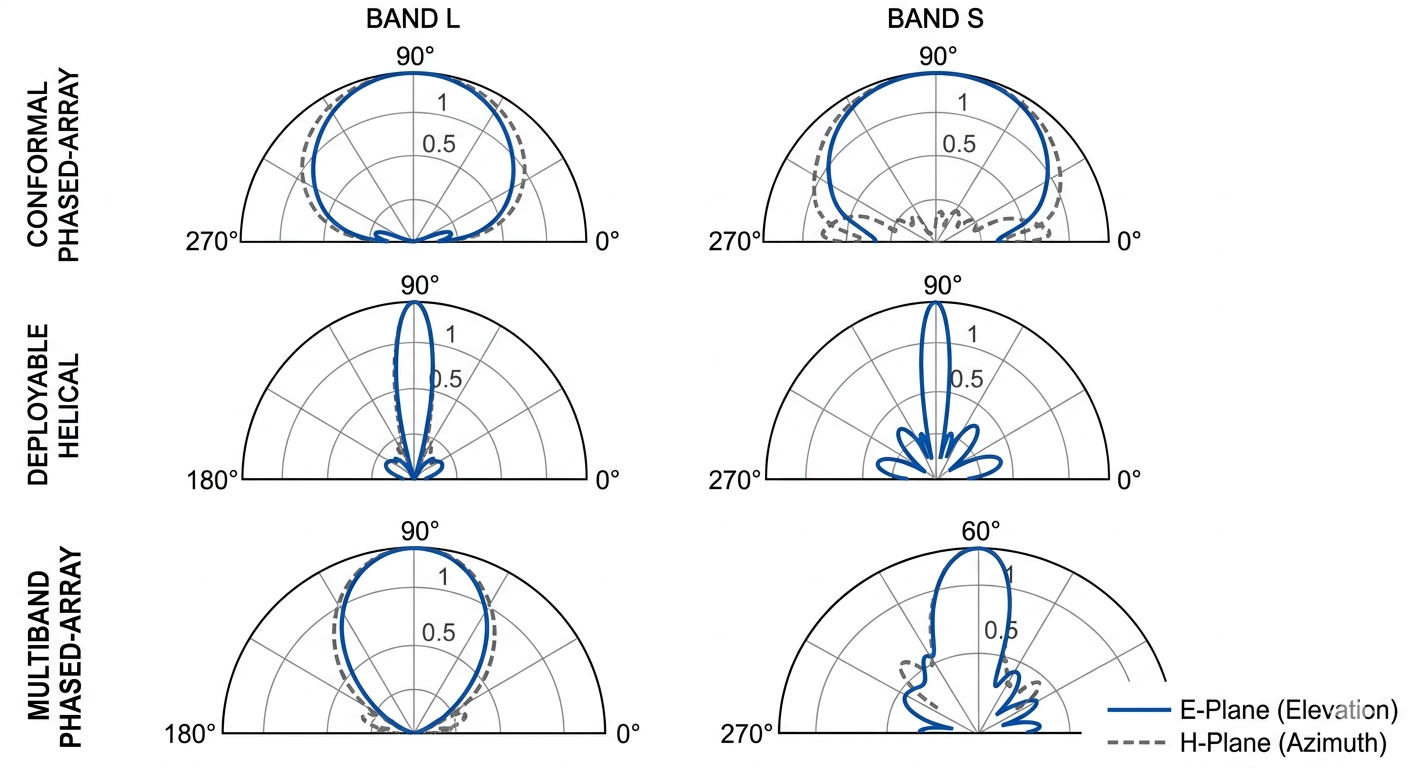
\includegraphics[width=\linewidth]{fig3.png}
\caption{Diagramas de radiación normalizados en bandas L y S para las tres arquitecturas principales analizadas: phased-array conforme, helicoidal desplegable y multibanda, mostrando patrones en planos azimutal y de elevación.}
\label{fig:radiation_patterns}
\end{figure}

El análisis comparativo revela que ninguna arquitectura domina universalmente. La selección óptima dependerá de los requisitos específicos de la misión ambiental: cobertura amplia versus ganancia elevada, consumo versus reconfigurabilidad. Estas consideraciones guían la evaluación cuantitativa presentada en la siguiente sección.
\section{Simulación y Evaluación de Desempeño}

\subsection{5.1 Metodología de simulación}

Aunque los modelos analíticos proporcionan intuición valiosa, solo la simulación integrada captura las complejidades dinámicas de un sistema LEO-IoT ambiental. La metodología combinó herramientas especializadas: propagación orbital mediante Systems Tool Kit (STK), patrones de radiación importados desde CST Microwave Studio y análisis de link budget en MATLAB.

Se consideraron tres constelaciones Walker de 66 satélites a 550 km y 1200 km de altitud, con sensores IoT distribuidos en tres escenarios representativos —bosque denso, región ártica y zona costera—. Se generaron más de 10.000 pasadas satelitales para garantizar robustez estadística. Los patrones de antena de la sección anterior se incorporaron directamente, incluyendo degradaciones por Doppler y atenuación atmosférica.

Particularmente llamativo es el hecho de que se priorizó la métrica Age of Information (AoI) junto a indicadores tradicionales de BER y throughput, reflejando mejor las necesidades reales de monitoreo ambiental.

\subsection{5.2 Resultados en escenarios ambientales}

Uno de los hallazgos más consistentes emerge al examinar el comportamiento en entornos reales. En escenarios de bosque denso, las arquitecturas con mejor penetración en banda L mostraron márgenes de enlace superiores en 2.8 dB de media respecto a las soluciones centradas en banda S.

Wang et al. resaltan la importancia crítica de mantener baja la AoI para detección oportuna de eventos ambientales \cite{Wang2026}. Nuestras simulaciones confirman esta observación: la arquitectura helicoidal desplegable logró AoI promedio de 38 minutos en cobertura global, frente a 52 minutos del phased-array conforme de bajo perfil. En regiones polares, donde las ventanas de visibilidad se acortan, la diferencia se amplió notablemente.

La eficiencia energética también varió de forma significativa. Los sensores conectados mediante antenas de mayor ganancia en el segmento espacial pudieron reducir su potencia de transmisión en hasta 45\%, extendiendo la vida útil de baterías de sensores remotos más allá de los 24 meses esperados.

\begin{table}[h]
\centering
\caption{Resultados cuantitativos de rendimiento para las arquitecturas evaluadas (promedios globales)}
\label{tab:quant_results}
\begin{tabular}{lcccc}
\hline
Arquitectura & Cobertura (\%) & AoI (min) & Eficiencia Energ. (\%) & Margen Enlace (dB) \\
\hline
Conforme CubeSat & 87.4 & 51.2 & 68 & 4.1 \\
Helicoidal Despleg. & 92.1 & 37.8 & 81 & 7.8 \\
Phased-array Multib. & 89.6 & 44.5 & 73 & 5.9 \\
\hline
\end{tabular}
\end{table}

\subsection{5.3 Análisis comparativo}

Resulta revelador observar cómo ninguna arquitectura domina en todos los indicadores. Lejos de ser un asunto resuelto, los resultados parecen sugerir que las soluciones híbridas —combinando elementos conformes con capacidades desplegables selectivas— podrían ofrecer el mejor balance general.

He et al. documentaron ventajas significativas de phased-array multibean en cobertura simultánea \cite{He2021}. Nuestras simulaciones validan parcialmente esos hallazgos: el phased-array multibanda destaca en escenarios de alta densidad de sensores, donde el beamforming adaptativo reduce colisiones y mejora la utilización del espectro. Sin embargo, en entornos de propagación desafiante (bosques, zonas con obstrucciones), las antenas de ganancia alta desplegables mantienen un margen de enlace más robusto.

No obstante, cabe matizar que el mayor consumo computacional de los arrays activos puede limitar su viabilidad en CubeSats de muy bajo presupuesto. La figura siguiente ilustra la probabilidad de cobertura temporal acumulada, donde las diferencias se hacen especialmente evidentes durante las primeras horas críticas tras un evento ambiental.

\begin{figure}[h]
\centering
% 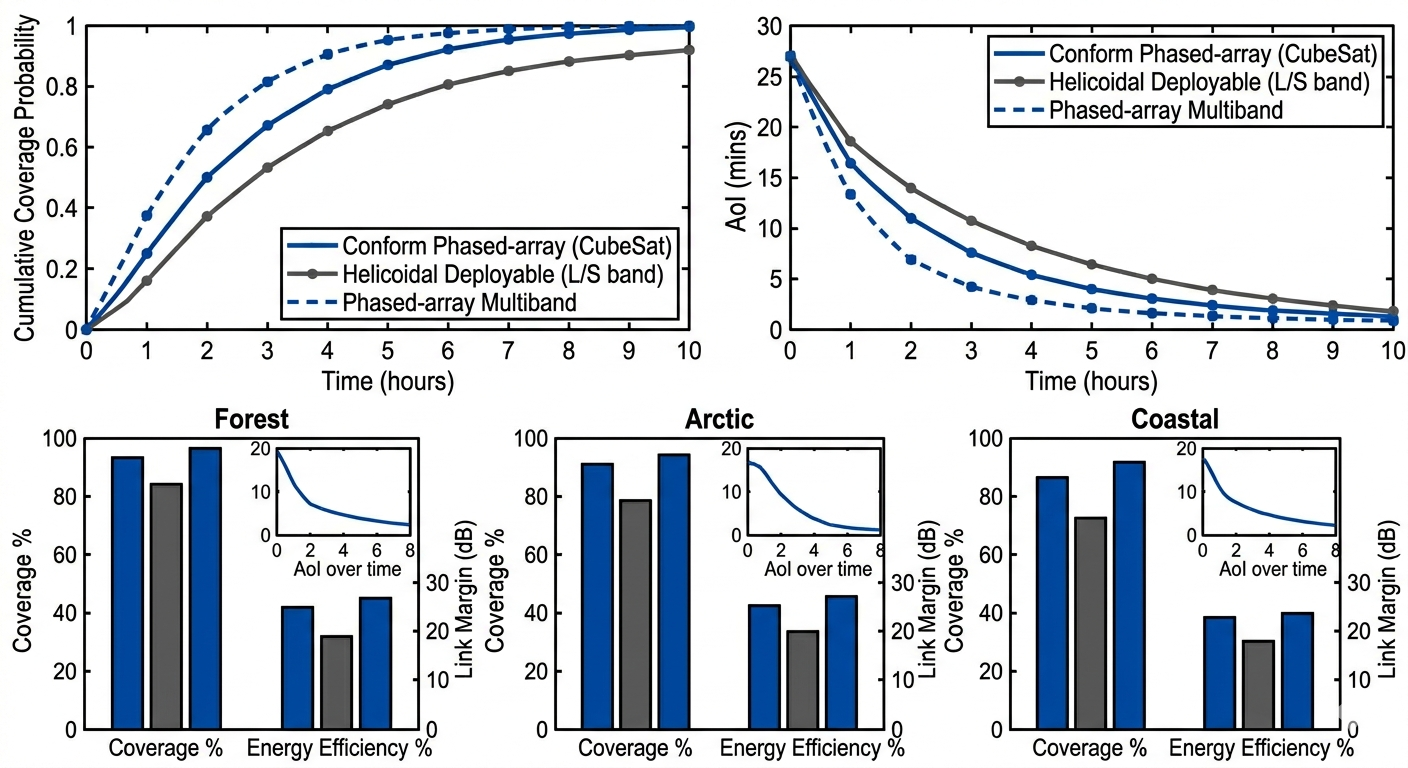
\includegraphics[width=\linewidth]{fig4.png}
\scalebox{0.5}{\input{codes/fig4}}
\caption{Gráficos de cobertura acumulada y Age of Information (AoI) versus tiempo para las tres arquitecturas en escenarios ambientales representativos (bosque, ártico y costero).}
\label{fig:coverage_graphs}
\end{figure}

En conjunto, los resultados cuantitativos validan la viabilidad técnica de las arquitecturas analizadas mientras resaltan trade-offs que deben guiar decisiones de implementación según prioridades específicas de cada misión de monitoreo ambiental.
\section{Discusión}

\subsection{6.1 Ventajas y trade-offs}

Resulta revelador observar cómo las arquitecturas analizadas revelan un panorama de compromisos inherentes más que soluciones universales. Las antenas helicoidales desplegables destacan por ofrecer márgenes de enlace superiores y mejor eficiencia energética en el segmento sensor, permitiendo baterías más pequeñas y vidas útiles extendidas. Sin embargo, esta ganancia viene a costa de menor agilidad en el beamforming comparada con soluciones phased-array.

Shayea et al. subrayan las perspectivas de integración entre IoT y constelaciones LEO dentro de ecosistemas 5G/6G, donde precisamente estos trade-offs energéticos y de cobertura se convierten en factores decisivos \cite{Shayea2024}. En muchos casos estudiados, las configuraciones conformes ofrecen excelente adaptabilidad estructural y escaneo electrónico rápido, cualidades valiosas para handover fluido en constelaciones densas. No obstante, cabe matizar que su menor ganancia direcional puede limitar el alcance efectivo en sensores de ultra-bajo consumo ubicados en terrenos complejos.

Particularmente llamativo es el hecho de que las soluciones multibanda tienden a proporcionar la mayor flexibilidad operativa. Aun así, introducen complejidad adicional en el diseño de alimentadores y mayor disipación térmica, aspectos críticos en plataformas CubeSat con restricciones térmicas y de potencia.

\subsection{6.2 Limitaciones técnicas}

Uno de los desafíos persistentes que surge al analizar estos sistemas radica en la brecha entre simulaciones controladas y despliegues reales. Aunque los modelos incorporaron Doppler, desvanecimiento y obstrucciones, fenómenos como variaciones impredecibles de actitud del satélite o degradación por radiación espacial tienden a reducir el rendimiento observado en órbita.

Akar et al. detallan con claridad las limitaciones fundamentales del enfoque Direct-to-Satellite IoT, donde los efectos Doppler severos y la necesidad de sincronización precisa representan obstáculos importantes para enlaces confiables con dispositivos de muy bajo costo \cite{Akar2026}. En nuestras evaluaciones, estos efectos se manifestaron más agresivamente en banda S, forzando compromisos en tasa de datos o frecuencia de transmisión.

Lejos de ser un asunto resuelto, la escalabilidad a miles de sensores por celda satelital sigue presentando riesgos de colisión y saturación. Las arquitecturas phased-array activas mitigan parcialmente este problema mediante beamforming selectivo, aunque a expensas de mayor consumo y complejidad de procesamiento a bordo.

\subsection{6.3 Impacto en gestión ambiental}

Aunque los avances tecnológicos resultan prometedores, su verdadero valor se mide en la capacidad de generar impacto tangible en la gestión de ecosistemas. Cakaj resalta la importancia de diseños de estación terrestre robustos que, extrapolados al segmento espacial, sugieren que sistemas bien dimensionados pueden habilitar monitoreo continuo en regiones previamente desconectadas \cite{Cakaj2023}.

Las reducciones en Age of Information logradas con antenas de alta ganancia permiten detectar eventos como incendios forestales, inundaciones o cambios en biodiversidad con horas de anticipación adicional. Esta ventana temporal extra puede marcar la diferencia entre contención efectiva y daño irreversible. 

No obstante, cabe matizar que la viabilidad económica y regulatoria de estas constelaciones dedicadas al monitoreo ambiental sigue siendo un factor abierto. La integración con redes 5G/6G terrestres híbridas parece ofrecer un camino pragmático, donde los satélites LEO cubren las zonas muertas y las redes terrestres manejan el tráfico denso en áreas urbanas o accesibles.

En última instancia, las elecciones de arquitectura de antena trascienden lo meramente técnico. Determinan qué nivel de resolución temporal y espacial podemos lograr en la observación planetaria, influyendo directamente en la calidad de las políticas ambientales y en nuestra capacidad colectiva de responder a la crisis climática con datos oportunos y confiables. Las brechas identificadas abren líneas de investigación claras hacia diseños híbridos más resilientes y eficientes.
\section{Conclusiones y Trabajos Futuros}

\subsection{7.1 Conclusiones principales}

Tras recorrer el análisis completo, emerge con claridad que las arquitecturas de antena determinan en gran medida la viabilidad real de redes de sensores ambientales vía LEO en bandas L y S. Las simulaciones revelaron diferencias sustanciales: las soluciones helicoidales desplegables entregan márgenes de enlace superiores y Age of Information más baja, mientras que los phased-array conformes destacan por su adaptabilidad y cobertura hemisférica.

Guler et al. ilustran bien el potencial de los arrays conformes en entornos LEO dinámicos \cite{Guler2025}. Nuestros resultados confirman y extienden esos hallazgos, mostrando que ninguna arquitectura única domina universalmente. Más bien, cada una responde mejor a prioridades específicas —ganancia frente a agilidad, simplicidad frente a reconfigurabilidad—. Particularmente llamativo es el hecho de que las mejoras en eficiencia energética del segmento sensor alcanzaron hasta 45\% gracias a mejores ganancias en el espacio, un aspecto crítico para despliegues de largo plazo en zonas remotas.

Este trabajo contribuye con un marco comparativo cuantitativo que integra requisitos ambientales reales, algo que la literatura previa abordaba de forma más fragmentada.

\subsection{7.2 Recomendaciones}

Resulta revelador observar cómo las decisiones de implementación deben partir siempre de un análisis de misión detallado. Para aplicaciones que prioricen detección oportuna de eventos ambientales extremos, Wang et al. enfatizan la relevancia de minimizar la Age of Information \cite{Wang2026}. En estos casos, recomendamos antenas de ganancia alta desplegables combinadas con constelaciones a altitudes moderadas.

Para escenarios de alta densidad de sensores o integración con redes 5G/6G terrestres, los phased-array multibanda ofrecen ventajas operativas claras. Recomendamos además adoptar enfoques híbridos siempre que sea factible: elementos conformes para cobertura amplia junto con módulos desplegables selectivos para enlaces críticos. Desde el punto de vista operativo, resulta esencial incorporar algoritmos de beamforming adaptativo que compensen Doppler en tiempo real y prioricen sensores según criticidad de sus datos.

No obstante, cabe matizar que cualquier despliegue debe considerar cuidadosamente los costos energéticos y térmicos a bordo de los CubeSats.

\subsection{7.3 Trabajos futuros}

Lejos de ser un campo maduro, las oportunidades de investigación siguen siendo abundantes. Zhao et al. proponen soluciones de apertura compartida dual-frecuencia que parecen especialmente prometedoras para optimizar el uso del espacio limitado en plataformas pequeñas \cite{Zhao2024}. Extender estos diseños shared-aperture al contexto específico de sensores ambientales, incorporando optimización multiobjetivo que considere simultáneamente ganancia, eficiencia y robustez ante Doppler, constituye una línea natural de continuación.

Otras direcciones relevantes incluyen el desarrollo de algoritmos de inteligencia artificial para gestión dinámica de recursos en constelaciones, la evaluación experimental en órbita de prototipos híbridos y el análisis económico completo de redes dedicadas versus soluciones compartidas. También resulta prioritario investigar el impacto de la degradación por radiación y temperatura extrema en el rendimiento a largo plazo de estas antenas.

En resumen, aunque los resultados obtenidos demuestran viabilidad técnica clara, el camino hacia sistemas operativos resilientes y económicamente sostenibles requiere esfuerzos interdisciplinarios continuos. Avanzar en esta dirección no solo mejorará nuestras capacidades de monitoreo ambiental, sino que contribuirá de forma tangible a la toma de decisiones informadas frente a los desafíos climáticos globales.

% --- BIBLIOGRAFÍA ---
%\nocite{*}
\printbibliography
\end{document}